% ROCODE (Jiang 2024) workflow figure.
% Synchronous compiler call at each statement boundary; on error,
% rollback to error line (first occurrence) or highest-entropy
% token (recurrence). lambda^(t-r) decaying penalty during regen.
\documentclass[border=2pt]{standalone}
\usepackage{tikz}
\usepackage{xcolor}
\usetikzlibrary{shapes.geometric, arrows.meta, positioning, fit, backgrounds, calc}

\begin{document}
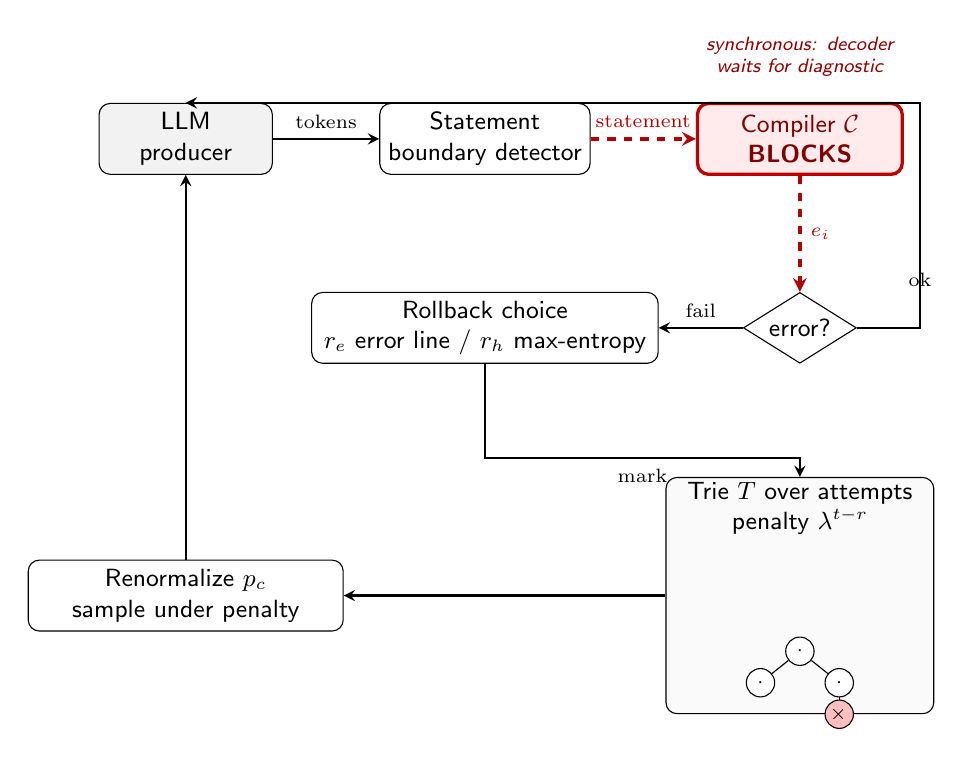
\begin{tikzpicture}[
    >=stealth,
    font=\sffamily\small,
    box/.style       ={draw, rounded corners, align=center, minimum height=9mm,
                       minimum width=26mm, inner sep=3pt, fill=white},
    llmbox/.style    ={box, fill=black!5, minimum width=22mm},
    blockbox/.style  ={box, draw=red!75!black, very thick, fill=red!8,
                       text=red!50!black, minimum width=26mm},
    trie/.style      ={box, fill=black!2, minimum width=34mm, align=center,
                       minimum height=30mm},
    decision/.style  ={diamond, draw, aspect=2.0, inner sep=1pt, align=center,
                       fill=white, minimum height=9mm},
    flow/.style      ={->, thick},
    blockflow/.style ={->, very thick, red!70!black, dashed},
    note/.style      ={font=\sffamily\scriptsize\itshape, text=red!55!black}
]

% Top row: LLM -> boundary -> compiler
\node[llmbox]   (llm) at (0,0) {LLM\\producer};
\node[box]      (bnd) at (3.8,0) {Statement\\boundary detector};
\node[blockbox] (cc)  at (7.8,0) {Compiler $\mathcal{C}$\\\textbf{BLOCKS}};

\node[note, above=2mm of cc, text width=32mm, align=center]
    {synchronous: decoder\\waits for diagnostic};

% Decision below compiler
\node[decision] (dec) at (7.8,-2.4) {error?};

% Rollback choice (below)
\node[box, minimum width=44mm] (rl) at (3.8,-2.4)
    {Rollback choice\\$r_e$ error line / $r_h$ max-entropy};

% Trie + penalty (bottom-right) -- box has space for the label on top
% and a small trie sketch beneath it.
\node[trie] (trie) at (7.8,-5.8) {};
\node[align=center, font=\sffamily\small]
    at ($(trie.north)+(0,-4mm)$) {Trie $T$ over attempts\\penalty $\lambda^{t-r}$};

% Mini trie sketch inside the trie box, lower portion.
\begin{scope}[shift={($(trie.south)+(0,8mm)$)}]
  \node[draw, circle, inner sep=0.6pt, minimum size=3.6mm, fill=white] (n0) at (0,0) {\scriptsize $\cdot$};
  \node[draw, circle, inner sep=0.6pt, minimum size=3.6mm, fill=white] (n1) at (-5mm,-4mm) {\scriptsize $\cdot$};
  \node[draw, circle, inner sep=0.6pt, minimum size=3.6mm, fill=white] (n2) at (5mm,-4mm)  {\scriptsize $\cdot$};
  \node[draw, circle, inner sep=0.6pt, minimum size=3.6mm, fill=red!25] (n3) at (5mm,-8mm) {\scriptsize \texttimes};
  \draw (n0)--(n1); \draw (n0)--(n2); \draw (n2)--(n3);
\end{scope}

% Resample box (bottom-left)
\node[box, minimum width=40mm] (resamp) at (0,-5.8)
    {Renormalize $p_c$\\sample under penalty};

% --- Arrows ---
\draw[flow] (llm.east) -- (bnd.west) node[midway, above, font=\scriptsize] {tokens};
\draw[blockflow] (bnd.east) -- (cc.west)
    node[midway, above, font=\scriptsize] {statement};

% Diagnostic returned
\draw[blockflow] (cc.south) -- (dec.north)
    node[midway, right, font=\scriptsize] {$e_i$};

% Error -> Rollback (left)
\draw[flow] (dec.west) -- (rl.east) node[midway, above, font=\scriptsize] {fail};

% OK branch -> back to LLM (right side, around)
\draw[flow] (dec.east) -- ++(8mm,0) |- (llm.north)
    node[pos=0.07, above, font=\scriptsize] {ok};

% Rollback -> Trie (downward)
\draw[flow] (rl.south) -- ++(0,-12mm) -| (trie.north)
    node[pos=0.25, below, font=\scriptsize] {mark};

% Trie -> resample
\draw[flow] (trie.west) -- (resamp.east);

% Resample -> LLM
\draw[flow] (resamp.north) -- (llm.south);

\end{tikzpicture}
\end{document}
